%%%%%%%%%%%%%%%%%%%%%%%%%%%%%%%%%%%%%%%%%
% Masters/Doctoral Thesis 
% LaTeX Template
% Version 2.4 (22/11/16)
%
% This template has been downloaded from:
% http://www.LaTeXTemplates.com
%
% Version 2.x major modifications by:
% Vel (vel@latextemplates.com)
%
% This template is based on a template by:
% Steve Gunn (http://users.ecs.soton.ac.uk/srg/softwaretools/document/templates/)
% Sunil Patel (http://www.sunilpatel.co.uk/thesis-template/)
%
% Template license:
% CC BY-NC-simulated annealing 3.0 (http://creativecommons.org/licenses/by-nc-sa/3.0/)
%
%%%%%%%%%%%%%%%%%%%%%%%%%%%%%%%%%%%%%%%%%

%--------------------------------------------
%	PACKAGES AND OTHER DOCUMENT CONFIGURATIONS
%--------------------------------------------

\documentclass[
11pt, % The default document font size, options: 10pt, 11pt, 12pt
%oneside, % Two side (alternating margins) for binding by default, uncomment to switch to one side
english, % ngerman for German
singlespacing, % Single line spacing, alternatives: onehalfspacing or doublespacing
%draft, % Uncomment to enable draft mode (no pictures, no links, overfull hboxes indicated)
%nolistspacing, % If the document is onehalfspacing or doublespacing, uncomment this to set spacing in lists to single
liststotoc, % Uncomment to add the list of figures/tables/etc to the table of contents
%toctotoc, % Uncomment to add the main table of contents to the table of contents
%parskip, % Uncomment to add space between paragraphs
%nohyperref, % Uncomment to not load the hyperref package
headsepline, % Uncomment to get a line under the header
%chapterinoneline, % Uncomment to place the chapter title next to the number on one line
%consistentlayout, % Uncomment to change the layout of the declaration, abstract and acknowledgements pages to match the default layout
]{MastersDoctoralThesis} % The class file specifying the document structure

% Encoding
\usepackage[utf8]{inputenc} % Required for inputting international characters
\usepackage[T1]{fontenc} % Output font encoding for international characters

% Bilbliography
\usepackage[style=numeric,natbib=true,giveninits=true,sorting=none]{biblatex}

% Document class "MasterDoctoralThesis" internals
\usepackage[autostyle=true]{csquotes} % Required to generate language-dependent quotes in the bibliography
\usepackage{import}
\usepackage{tocbibind}

% Images
\usepackage{graphicx} % Permet l'insertion d'image (entre autres)
\usepackage{pict2e} % Pour faire des graphiques

% Tikz and colors
\usepackage{color}
\usepackage{xcolor}
\usepackage{tikz}
	\usetikzlibrary{patterns}
	\usetikzlibrary{plotmarks}
	\usetikzlibrary{calc}
	\usetikzlibrary{shapes}
	\usetikzlibrary{arrows}
	\usetikzlibrary{fadings}

% Maths
\usepackage{amsmath} % Mathematical environnements
\usepackage{amsfonts} % Mathematical fonts
\usepackage{amssymb} % Mathematical symbols

% Tables and figures
\usepackage{array} % For tables
\usepackage{floatrow} % ??
\usepackage{subfig} % Subfigure possible
\usepackage{tabu} % Better tabular

% Misc
\usepackage[english]{babel}
\usepackage{verbatim} % Verbatim
\usepackage{bbm} % Extended blackboard bold symbols
\usepackage[colorinlistoftodos, obeyFinal]{todonotes}
\usepackage{xspace} % Trailing space for custom commands
\usepackage{hyperref}
\hypersetup{
    colorlinks,
    linkcolor={red!50!black},
    citecolor={blue!50!black},
    urlcolor={blue!80!black}
}

% Showlabel
\usepackage{showlabels}

\renewcommand{\showlabelfont}{\tiny\color{blue}}
\renewcommand{\showlabelsetlabel}[1]{\colorbox{lightgray}{\showlabelfont #1}}

% Setup
\floatsetup[figure]{style=plain,subcapbesideposition=top}
\addbibresource{biblio.bib} % The filename of the bibliography

% Options
\usepackage{palatino} % Use the Palatino font by default

\usepackage[draft]{showlabels}

\renewcommand{\showlabelfont}{\tiny\color{blue}}
\renewcommand{\showlabelsetlabel}[1]{\colorbox{lightgray}{\showlabelfont #1}}

\floatsetup[figure]{style=plain,subcapbesideposition=top}

%--------------------------------------------
%   CUSTOM COMMANDS
%--------------------------------------------
\newcommand{\bigO}[1]{\mathcal{O}\left(#1\right)} % big O notation
\newcommand{\code}[1]{\texttt{#1}} % shortcut to insert code inline
\newcommand{\EE}[1]{\cdot 10^{#1}} % power of 10
\newcommand{\missingref}{[\todo[color=blue!30, size=\tiny, caption={Missing reference}]{Missing ref}?]\xspace}
\newcommand{\myvec}[1]{\boldsymbol{\mathrm{#1}}} % bold vectors
\newcommand{\norm}[1]{\Vert #1\Vert} % norm of a vector
\newcommand{\set}[1]{\{#1\}} % set notation with curly braces
\newcommand{\total}{\text{d}} % d for total derivative


% Project specific

\newcommand{\lambdavec}{\myvec{\lambda}}
\newcommand{\uvec}{\myvec{u}}

\makeatletter

\def\@setref#1#2#3{%
  \ifx#1\relax
   \protect\G@refundefinedtrue
   \nfss@text{\reset@font\bfseries\tiny\textcolor{red}{Ref to \colorbox{lightgray}{\texttt{#3}}}}%
   \@latex@warning{Reference `#3' on page \thepage \space
             undefined}%
  \else
   \expandafter#2#1\null
  \fi}

\makeatother


%--------------------------------------------
%	MARGIN SETTINGS
%--------------------------------------------

\geometry{
	paper=a4paper, % Change to letterpaper for US letter
	inner=2.5cm, % Inner margin
	outer=3.8cm, % Outer margin
	bindingoffset=.5cm, % Binding offset
	top=1.5cm, % Top margin
	bottom=1.5cm, % Bottom margin
	%showframe, % Uncomment to show how the type block is set on the page
}

%--------------------------------------------
%	THESIS INFORMATION
%--------------------------------------------

\thesistitle{Giant connected component in networks} % Your thesis title, this is used in the title and abstract, print it elsewhere with \ttitle
\supervisor{Dr. Guiyuan \textsc{SHI}\\Prof. Yi-Cheng \textsc{Zhang}} % Your supervisor's name, this is used in the title page, print it elsewhere with \supname
\examiner{} % Your examiner's name, this is not currently used anywhere in the template, print it elsewhere with \examname
\degree{Master Project} % Your degree name, this is used in the title page and abstract, print it elsewhere with \degreename
\author{Benoît \textsc{Richard}} % Your name, this is used in the title page and abstract, print it elsewhere with \authorname
\addresses{} % Your address, this is not currently used anywhere in the template, print it elsewhere with \addressname

\subject{Physics} % Your subject area, this is not currently used anywhere in the template, print it elsewhere with \subjectname
\keywords{} % Keywords for your thesis, this is not currently used anywhere in the template, print it elsewhere with \keywordnames
\university{University of Fribourg} % Your university's name and URL, this is used in the title page and abstract, print it elsewhere with \univname
\department{Department of Physics} % Your department's name and URL, this is used in the title page and abstract, print it elsewhere with \deptname
\group{Theoretical Interdisciplinary Physics Group} % Your research group's name and URL, this is used in the title page, print it elsewhere with \groupname
\faculty{Faculty of Science} % Your faculty's name and URL, this is used in the title page and abstract, print it elsewhere with \facname

\AtBeginDocument{
\hypersetup{pdftitle=\ttitle} % Set the PDF's title to your title
\hypersetup{pdfauthor=\authorname} % Set the PDF's author to your name
\hypersetup{pdfkeywords=\keywordnames} % Set the PDF's keywords to your keywords
}

\begin{document}

\frontmatter % Use roman page numbering style (i, ii, iii, iv...) for the pre-content pages

\pagestyle{plain} % Default to the plain heading style until the thesis style is called for the body content

%--------------------------------------------
%	TITLE PAGE
%--------------------------------------------

\begin{titlepage}
\begin{center}

\vspace*{.06\textheight}
{\scshape\LARGE \univname\par}\vspace{1.5cm} % University name
\textsc{\Large Master Project}\\[0.5cm] % Thesis type

\HRule \\[0.4cm] % Horizontal line
{\huge \bfseries \ttitle\par}\vspace{0.4cm} % Thesis title
\HRule \\[1.5cm] % Horizontal line
 
\begin{minipage}[t]{0.4\textwidth}
\begin{flushleft} \large
\emph{Author:}\\
\authorname
\end{flushleft}
\end{minipage}
\begin{minipage}[t]{0.4\textwidth}
\begin{flushright} \large
\emph{Supervisors:} \\
\supname
\end{flushright}
\end{minipage}\\[3cm]
 
\vfill

\large \textit{}\\[0.3cm] % University requirement text
\textit{}\\[0.4cm]
\groupname\\\deptname\\[2cm] % Research group name and department name
 
\vfill

{\large \today}\\[4cm] % Date
%\includegraphics{Logo} % University/department logo - uncomment to place it
 
\vfill
\end{center}
\end{titlepage}

%--------------------------------------------
%	ABSTRACT PAGE
%--------------------------------------------

\begin{abstract}
\addchaptertocentry{\abstractname} % Add the abstract to the table of contents
\todo[inline]{Write the abstract}
\end{abstract}

%--------------------------------------------
%	LIST OF CONTENTS/FIGURES/TABLES PAGES
%--------------------------------------------

\tableofcontents % Prints the main table of contents

% \listoffigures % Prints the list of figures

% \listoftables % Prints the list of tables

%--------------------------------------------
%   ABBREVIATIONS
%--------------------------------------------

%\begin{abbreviations}{ll} % Include a list of abbreviations (a table of two columns)

%\end{abbreviations}

%--------------------------------------------
%	SYMBOLS
%--------------------------------------------

\begin{symbols}{m{0.1\textwidth}m{0.6\textwidth}m{0.25\textwidth}} % Include a list of Symbols (a two column table)

\textbf{Symbol}	& \textbf{Description} & \textbf{Math. definition} \\
\addlinespace

$\deg(v)$	& Degree of vertex $v$ \\
$g_0(z)$	& Generating function for the degree of uniformly chosen nodes & $\sum_{k=0}^\infty p_k z^k$ \\
$g_1(z)$	& Generating function for the degree of nodes reached by following an edge & $\sum_{k=0}^\infty q_k z^k$ \\
$n$			& Number of nodes in the network \\
$N(v)$ 		& Neighborhood of a vertex $v$ \\
$p_k$		& Probability that a random node has degree $k$ & $P_0(\deg(v) = k)$ \\
$P_0$		& Probability starting from a uniformly chosen node \\
$P_1$		& Probability starting from a node reached by following an edge \\
$q_k$		& Probability that a node reached by following a edge has degree $k$ & $P_1(\deg(v) = k)$ \\
$S$ 		& Fraction of the network which is part of the GCC in the large $n$ limit & $P_0(v \in GCC)$ \\
$u$			& Probability that a node reached by following an edge from is not part of the GCC & $P_1(v \notin GCC)$ \\

\addlinespace
\addlinespace
\addlinespace

$g^{(i)}_0(z)$		& Generating function for the degree of uniformly chosen nodes in layer $i$ \\
$g^{(i)}_1(z)$		& Generating function for the degree of nodes reached by following an edge in layer $i$ \\
$p^{(i)}_k$			& Probability that a uniformly chosen node has degree $k$ in layer $i$ \\

\end{symbols}



%--------------------------------------------
%	THESIS CONTENT - CHAPTERS
%--------------------------------------------

\mainmatter % Begin numeric (1,2,3...) page numbering

\pagestyle{thesis} % Return the page headers back to the "thesis" style

%--------------------------------------------
%	INTRODUCTION
%--------------------------------------------
\listoftodos

\chapter{Introduction}

Many systems in real world can be conceptually represented as objects being connected to others. Such representation is called a network. For example, a road network can be represented as a set of crossings that are connected by direct roads. However, the concept of network does not require the object or the link between them to be physical. We can represent friendship relations as a network: two people are connected if they consider to be friends.

Mathematically, networks are represented as \emph{graphs}. A graph is an object composed of a set $V$ of nodes (also referred to as vertices) and a set of edges $E$. An edge is characterized by the fact that it connects two nodes together, which in mathematical terms translate to the fact that an edge can be written as a pair of nodes or equivalently $E \subset \set{(v_1, v_2) | v_1, v_2 \in V }$. To fit the numerous systems many extension of this simple model can be considered, for example edges may have a direction (\emph{directed graph}), meaning that $(v_1, v_2) \neq (v_2, v_1)$, edges or vertices can also have carry a value (\emph{weighted graph}) or multiple edges between two vertices may be allowed.

\todo[inline]{Introduce generating functions}


%--------------------------------------------
%	SINGLE LAYER
%--------------------------------------------
\chapter{Single layer networks}

Single layer networks correspond to the classic picture of a network.

\section{Configuration model}

Rather than studying peculiar and unique networks, we would like to  find properties of whole classes of networks. This allows to average properties over such network classes and thus may allow to identify characteristics fundamental to the network structure.

Since we would like to consider classes of network, we must first classify them. A common and useful\todo{add ref} way of doing so is to consider that two networks are element of the same class $\Omega$ if they have the same set of degrees. This definition is useful for two main reasons. First, the set of degrees of a network is easily measured if its structure is known. Second it is possible to generate a random network uniformly chosen in its class using the so called \emph{configuration model}. The main goal of this section is to describe the configuration model and how it achieves this.

Consider a network with $n$ vertices with degrees $d_i$, $i = 1 \dots n$. If we cut every edges in two then every vertex will be disconnected from the other and keep a number of "half edges" equal to its degree. In the context of the configuration model, we call such "half edge" a \emph{stub}. The resulting set of vertices and stub is independent of the network structure, but common for all networks with the same degree distribution. The idea of the configuration model is thus to start from this state and bond stubs two by two in a meaningful way to recreate edges of the network.

It appears that a good way to choose which stubs to bond together is to uniformly pick two amongst all of them. This procedure is good in the sense that it generate a network uniformly chosen in the class $\Omega$ of the network.

\todo[inline]{Network distribution and multi- and self-edges distribution}

\section{Giant connected component}

An interesting property of a network is the presence and size of \emph{connected component}. A set of nodes is said to be connected if there is a path of edges from any of its node to any other. All networks can divided in connected components such that all nodes are element of exactly one component, as can be seen on fig. \ref{Figure: Connected components}. The connectedness of network is crucial in many real world realisations of networks. In particular any logistic network, such as power grid networks, rail road network or the internet network, is functional only if it is able to transfer goods or services (electricity, passengers or informations) from any node to any other.

\begin{figure}
	\missingfigure{Connected component}
	\caption{}
	\label{Figure: Connected components}
\end{figure}

As we will see in section \ref{Section: Degree distribution in the GCC}, it is really hard to generate a fully connected network chosen uniformly in its class. A simpler, yet powerful approach, is to instead consider the biggest connected part of a network generated using the configuration model. This component, if its relative size does not vanish in the limit of large $n$, is called the \emph{giant connected component} (GCC). The first question is: what will be the size of the giant connected component ?

To determine this we first define $u$ the probability that a node reached by following an edge is not part of the GCC. We can therefore write the probability $S$ that a randomly chosen vertex is part of the GCC as
\begin{align}
	S 	&= 1 - P_0(w \notin GCC\; \forall w \in N(v))\\
		&= 1 - \sum_{k=0}^\infty P_0(w \notin GCC\; \forall w \in N(v)|\deg(v) = k) P_0(\deg(v) = k) \\
		&= 1 - \sum_{k=0}^\infty \left[P_1(w \notin GCC)\right]^k p_k \\
		&= 1 - \sum_{k=0}^\infty u^k p_k \\
		&= 1 - g_0(u).
\end{align}
We have now a compact expression for $S$ in terms of $u$ and the generating function of the degree distribution $g_0$. To determine $u$ we notice that if a vertex is not part of the GCC, none of its neighbors is. This allows to write
\begin{align}
	u 	&= P_1(w \notin GCC \; \forall w \in N(v)) \\
		&= \sum_{k=0}^\infty P_1(w \notin GCC \; \forall w \in N(v)| \deg(v) = k) P_1(\deg(v) = k) \\
		&= \sum_{k=0}^\infty u^k q_k \\
		&= g_1(u).
\end{align}
We end up with two equations to describe the GCC size
\begin{align}
	S = 1 - g_0(u) \label{Single layer GCC final} \\
	u = g_1(u). \label{Single layer u final}
\end{align}
If we can solve the second one we immediately get the GCC size. However eq. \eqref{Single layer GCC final} only gives $u$ implicitly and its form strongly depends on the degree distribution, therefore no general analytical solutions can be given. A particular solution is however always present for $u = 1$ as by definition \todo{Add reference to definition of g1} $g_1(1) = 1$. This implies $S = 0$ and thus the absence of GCC.

\todo[inline]{Add discussion/proof of existence of GCC when multiple solutions are present ?}

\begin{figure}
	\missingfigure{$u = g_1(u)$ graphically}
	\caption{}
\end{figure}

{\floatsetup[figure]{style=plain,subcapbesideposition=center}
\begin{figure}
	\sidesubfloat[]{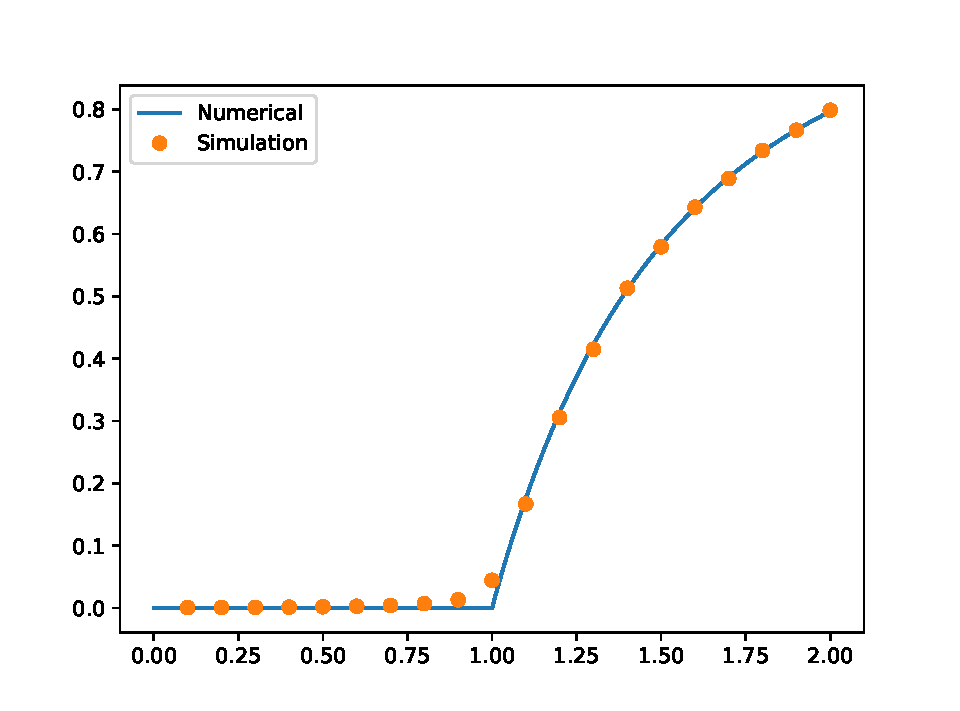
\includegraphics[width=0.8\textwidth]{numerical_simulation_one_layer_poisson.pdf}}\\
	\sidesubfloat[]{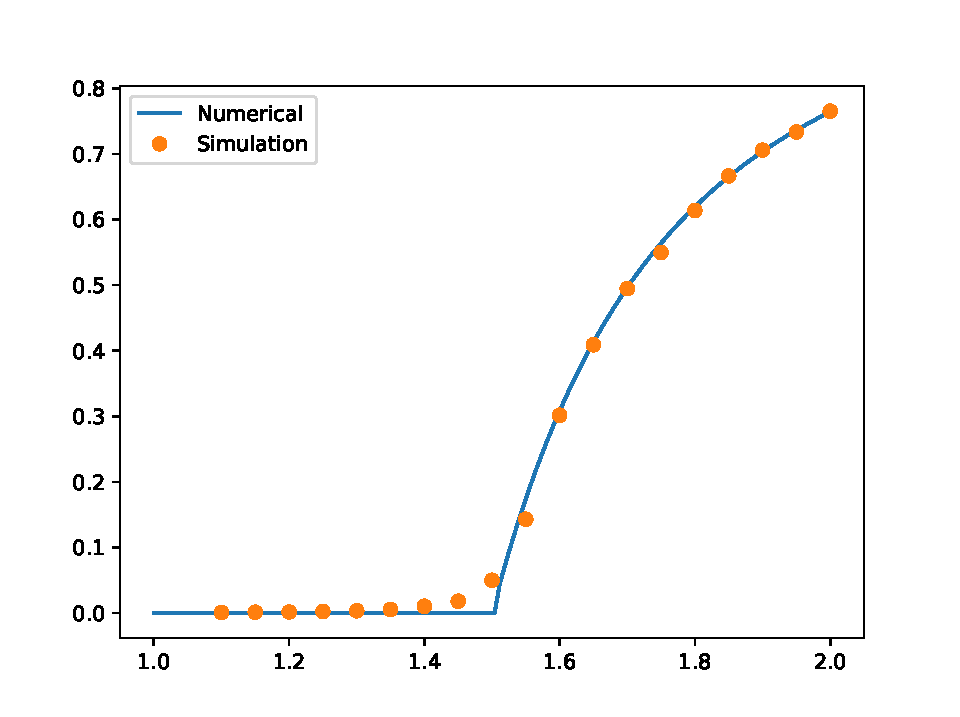
\includegraphics[width=0.8\textwidth]{numerical_simulation_one_layer_geometric.pdf}}
	\caption{Numerical solution of eqs. \eqref{Single layer GCC final} and \eqref{Single layer u final}, together with results on simulated networks. Results of simulations are average over 10 runs and the network size was set to $10^4$ nodes. Simulations ran for several seconds in total, indicating that much larger network should be easily usable. (A) Poisson degree distribution. (B) Geometric degree distribution.}
\end{figure}
}

\newpage



\section{Degree distribution in the GCC}
\label{Section: Degree distribution in the GCC}

Per Bayes theorem we have for two event $A$ and $B$
\begin{align}
	P(A | B) = \frac{P(A \cap B)}{ P(B)} = P(B | A) \frac{P(A)}{P(B)}. \label{Bayes theorem}
\end{align}
This allows us to compute the degree distribution of the vertices in the giant connected component
\begin{align}
	P(deg(v) &= k | v \in GCC) = P(v \in GCC | deg(v) = k) \frac{P(deg(v) = k)}{P(v \in GCC)} \\
	&= (1 - P(v \notin GCC|deg(v) = k)) \frac{p_k}{S} \\
	&= \frac{p_k}{S} (1 - u^k). \label{Degree distribution in GCC}
\end{align}

\begin{figure}
	\missingfigure{low degree saturation in GCC}
\end{figure}

By multiplying this expression by $z^k$ for each $k$ and summing, we find the generating function $G_0(z)$ of the degree distribution in the giant connected component
\begin{align}
	G_0(z) = \frac{1}{S} (g_0(z) - g_0(u z)).
\end{align}


\chapter{Multiplex network}

\section{Giant viable cluster}

Consider a multiplex network with $L$ layers. Let $g_0^{(i)}$ and $g_1^{(i)}$ be the generating functions of respectively the degree and the excess degree in layer $i$. Moreover define $u_i$ as the probability that a vertex reached after following an edge in layer $i$ is not part of the giant viable cluster. Then if we pick a vertex $v$ at random the probability $S$ that it is part of the giant viable cluster can be written as
\begin{align}
	S &= P_0\left(\bigcap_{i = 1}^{L} \exists w \in N_i(v) \; w \in GVC \right).
\end{align}
By requiring that the layers are independent from one others, we can rewrite $S$ as a product
\begin{align}
	S &= \prod_{i = 1}^{L}  P_0\left(\exists w \in N_i(v) \; w \in GVC\right) \\
		&=\prod_{i = 1}^{L}  \left[1 - P\left(w \notin GVC \; \forall w \in N_i(v)\right) \right] \\
		&=\prod_{i = 1}^{L}  \left[1 - \sum_{k = 0}^{\infty} P\left((w \notin GVC \; \forall w \in N_i(v) | deg(v) = k \right) p^{(i)}_k \right] \\
		&=\prod_{i = 1}^{L}  \left[1 - \sum_{k = 0}^{\infty} u_i^k p^{(i)}_k \right] \\
		&=\prod_{i = 1}^{L}  \left[1 - g_0^{(i)}(u_i) \right].\label{Multiplex GCC size final}
\end{align}

We can find $u_j$ by a similar reasoning. First note that $1 - u_j$ is the probability that a vertex reached by following an edge in layer $j$ is in the giant viable cluster. Which as before can be written in the form
\begin{align}
	1 - u_j &= P_1^{(j)}\left(\bigcap_{i = 1}^{L} \exists w \in N_i(v) \; w \in GVC\right)\\
	&= \prod_{i = 1}^{L}  P_1^{(j)}\left(\exists w \in N_i(v) \; w \in GVC \right).
\end{align}
Since the layers are independent, the fact that we reached $v$ by following an edge in layer $j$ to reach vertex $v$ is irrelevant in all other layers. However in layer $j$ this means that the degree distribution follows the distribution $q_k^{(j)}$ rather than $p_k^{(j)}$. Putting this together we get
\begin{align}
	1 - u_j &= \left[1 - \sum_{k = 0}^{\infty} u_j^k q_k^{(j)} \right] \prod_{\substack{i = 1 \\ i \neq j}}^{L}  \left[1 - \sum_{k = 0}^{\infty} u_i^k p^{(i)}_k \right] \\
	&= \left[1 - g_1^{(j)}(u_j) \right] \prod_{\substack{i = 1 \\ i \neq j}}^{L}  \left[1 - g_0^{(i)}(u_i) \right]. \label{Multiplex u final}
\end{align}

{\floatsetup[figure]{style=plain,subcapbesideposition=center}
\begin{figure}
	\sidesubfloat[]{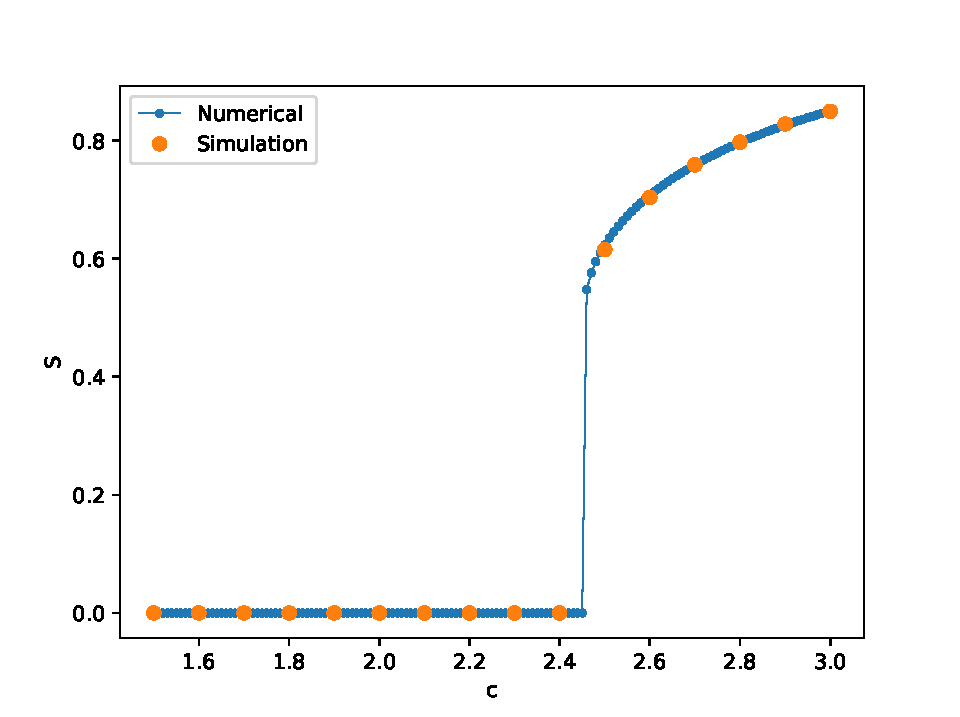
\includegraphics[width=0.8\textwidth]{numerical_simulation_double_layer_poisson_equal_c.pdf}}\\
	\sidesubfloat[]{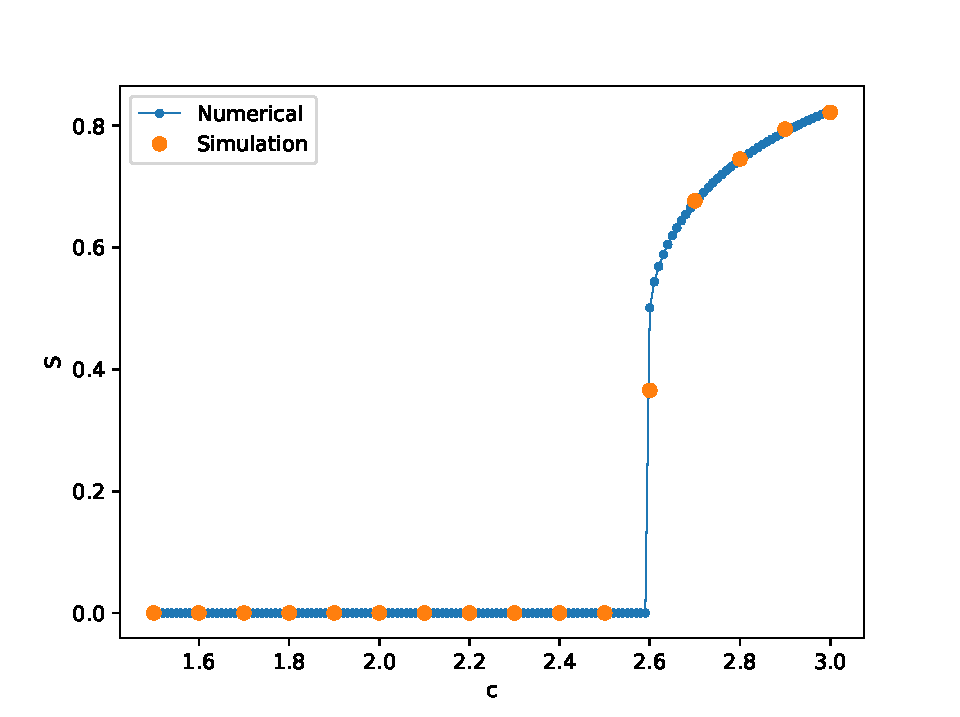
\includegraphics[width=0.8\textwidth]{numerical_simulation_double_layer_geometric_equal_c.pdf}}
	\caption{Numerical solution of eqs. \eqref{Multiplex GCC size final} and \eqref{Multiplex u final}, together with results on simulated networks for multiplex networks composed of two layers with the same distribution and mean number of edge $c$. Results of simulations are average over 10 runs and the network size was set to $10^4$ nodes. Simulations ran for several seconds in total, indicating that much larger network should be easily usable. (A) Poisson degree distribution. (B) Geometric degree distribution.}
\end{figure}
}

\newpage

\section{Boundary condition}

Equations \eqref{Multiplex GCC size final} and \eqref{Multiplex u final} are in principle sufficient to determine the size $S$ of the giant viable cluster in a multiplex network. We see that there always exists a trivial solution
\begin{align}
	u_j &= 1, \qquad \forall j,\\
	S &= 0.
\end{align}
Moreover this is the only solution for which $S = 0$. Indeed since $g_0^{(j)}$ is a strictly increasing function, we have
\begin{align}
	g_0^{(j)}(z) = 0 \quad \Leftrightarrow \quad z = 1.
\end{align}
So if $S = 0$, there exists $k$ such that $u_k = 1$. If we put it back in eq. \eqref{Multiplex u final}, it forces $1 - u_j = 0$ for all $j$, and thus all $u_j$ are one.

\todo[inline]{Something about the fact that the degree distributions are determined by some set of parameters $\lambda_j$}

We now introduce the following notations:
\begin{align}
	\uvec &= (u_1, u_2, \dots, u_L) \\
	\lambdavec &= (\lambda_1, \lambda_2, \dots, \lambda_N) \\
	f_j(\lambdavec, \uvec) &= 1 - u_j - \left[1 - g_1^{(j)}(u_j) \right] \prod_{\substack{i = 1 \\ i \neq j}}^{L}  \left[1 - g_0^{(i)}(u_i) \right] \label{Definition fj}
\end{align}
and the function
\begin{align}
	F : \mathbb{R}^N \times D_L &\rightarrow \mathbb{R}^L \\
	(\lambdavec, \uvec) &\mapsto F(\lambdavec, \uvec) = (f_1(\lambdavec, \uvec), f_2(\lambdavec, \uvec), \dots, f_L(\lambdavec, \uvec)), \label{Definition F}
\end{align}
where $D_L = [0, 1]^L$. Since the $g_0^{(i)}$ and $g_1^{(i)}$ are analytic with respect to the $u_i$, the function
\begin{align}
	F_{\lambdavec} : D_L &\rightarrow \mathbb{R}^L\\
		\uvec &\mapsto F_{\lambdavec}(\uvec) = F(\lambdavec, \uvec),
\end{align}
for a given parameter vector $\lambda$ is continuously differentiable as well. Therefore we can define its Jacobi matrix $J(\lambdavec, \uvec)$ as having coefficients
\begin{align}
	\left[ J(\lambdavec, \uvec) \right]_{ij} = \frac{\partial f_i(\lambdavec,\uvec)}{\partial u_j}.
\end{align}

In terms of the introduced notation, solving eq. \eqref{Multiplex u final} is equivalent to finding $\uvec^*$ such that
\begin{align}
	F(\lambdavec, \uvec^*) = 0.
\end{align}

If we assume that $F$ (and not only $F_{\lambdavec}$) is continuously differentiable and that we know a solution $\uvec^*$ for some parameter vector $\lambdavec^*$, we can use the implicit function theorem which give us the following:

If $\det\left[ J(\lambdavec, \uvec^*) \right] \neq 0$ then there is an open neighbourhood $U \subset \mathbb{R}^L$ of $\lambdavec^*$ such that there is an unique continuously differentiable function $g : U \rightarrow D_L$ with
\begin{align}
	g(\lambdavec^*) &= \uvec^* \\
	F(\lambdavec, g(\lambdavec)) &= 0, \quad \forall \lambdavec \in U. \label{Implicit solution for F}
\end{align}
In other words, we can express the solution $\uvec^*$ of eq. \eqref{Multiplex u final} in terms of the parameter vector $\lambdavec$ as $\uvec^* = g(\lambdavec)$.

The interesting result however comes from the contrapositive statement, namely that if we can not find a proper neighbourhood $U$ and function $g$, then the determinant of the Jacobi matrix$J(\lambdavec, \uvec)$ must be zero. This can append for two reasons.

First, for any neighbourhood $U$ of $\lambdavec^*$ the function $g$ is not uniquely define. This implies that for any neighbourhood $U$ of $\lambdavec^*$ there are  $g_1$ and $g_2$ continuously differentiable with
\begin{align}
	g_1(\lambdavec^*) &= g_2(\lambdavec^*) = \uvec^* \\
	F(\lambdavec, g_1(\lambdavec)) &= F(\lambdavec, g_2(\lambdavec)) =  0, \quad \forall \lambdavec \in U.
\end{align}
and that there is $\myvec{\lambda^\dagger} \in U$ such that $g_1(\myvec{\lambda^\dagger}) \neq g_2(\myvec{\lambda^\dagger})$. Therefore $\lambdavec^*$ is a critical point for a continuous phase transition. \todo{More explanation of this fact}

The other case is that for any neighbourhood $U$ of $\lambdavec^*$ any function $g$ defined on $U$ with $g(\lambdavec^*) = \uvec^*$ will either not be continuously differentiable or not fulfil eq. \eqref{Implicit solution for F}. In both cases, this correspond to $\lambdavec^*$ being a critical point of a discontinuous phase transition.\todo{Verify and be more explicit}

Therefore, in any cases where $\det\left[ J(\lambdavec^*, \uvec^*) \right] = 0$ and $F(\lambdavec^*, \uvec^*) = 0$, $\lambdavec^*$ is a critical point of the system. The condition on the determinant of the Jacobi matrix is thus in principle sufficient to determine the set of critical points.

%--------------------------------------------
%	THESIS CONTENT - APPENDICES
%--------------------------------------------

\appendix % Cue to tell LaTeX that the following "chapters" are Appendices


%--------------------------------------------
%	BIBLIOGRAPHY
%--------------------------------------------

\printbibliography[heading=bibintoc]

%--------------------------------------------

\end{document}